\chapter{Network Theory}
\label{ch:networktheory}

\begin{chapterabstract}
The theory underpinning complex networks is discussed, covering the representation of atomic systems as networks and the relationship of the dual network to ring structure.
The laws which govern the topological properties of physical networks are also introduced, namely Euler's law (mean node degree), \lm's law (node degree distribution) and the \aw{} law (node degree correlations).
\end{chapterabstract}

\section{Network Theory}
\label{sec:networktheory}

The scope of what constitutes a complex network is extremely broad, covering everything from the tangible (\eg{} computational clusters) to the more abstract (\eg{} social interactions). Yet part of the appeal and power of network science is the ability to quantify and relate these highly disparate systems with the same underlying theory.
A network is simply a collection of components termed \textit{nodes} and the connections between them termed \textit{links}, an example of which is given in figure \ref{fig:smallnet}.
There are then two fundamental classes of network based on the nature of the connections.
Networks in which the links between nodes are mutual are termed undirected, whereas those in which the links are one\--way are termed directed \cite{barabasi2016n}.
At the risk of dating this thesis, this is the difference between Facebook (an undirected social network of friends) and Twitter (a directed social network of followers).
All the networks considered in this work are undirected and all the theory assumes this property.

\begin{figure}[ht]
     \centering
      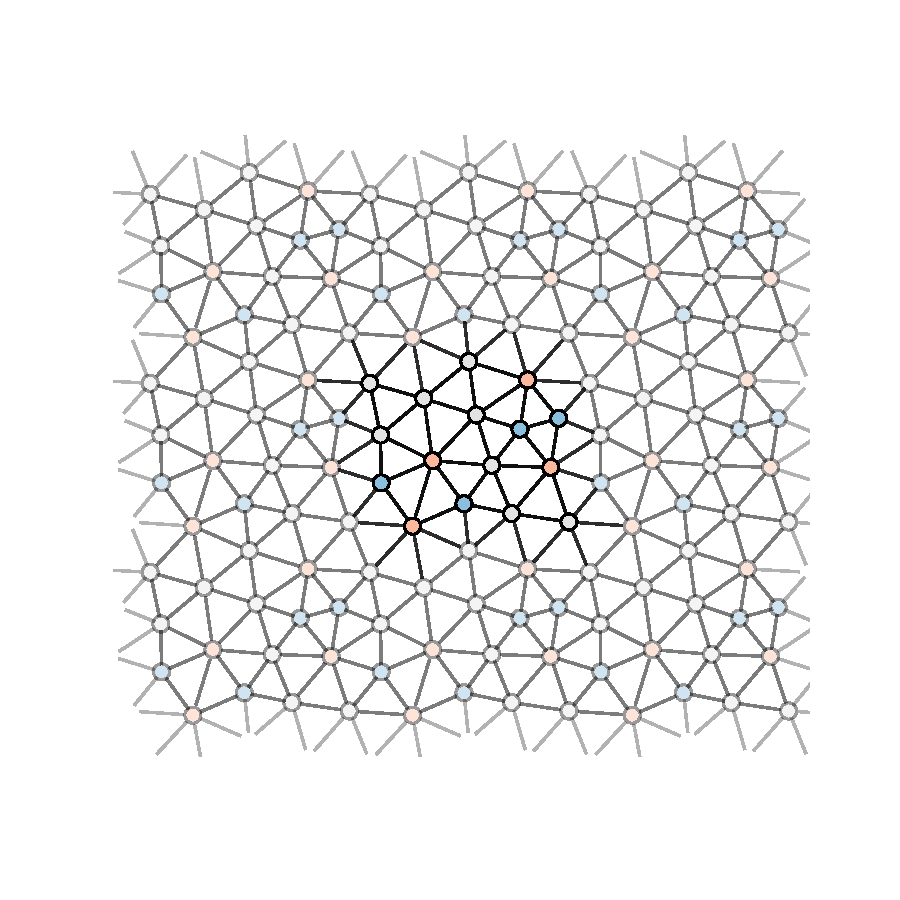
\includegraphics[width=8cm]{./figures/methods/small_periodic_net.pdf}
     \caption{Example of a periodic \td{} network where nodes are represented by circles and links as lines. Nodes are coloured similarly according to their degree, whilst periodic images are greyed out to highlight the central repeating unit.}
     \label{fig:smallnet}
\end{figure}

\subsection{Node Degree and Probability Distributions} 
\label{s:theorynodeprob}

A key concept in network science is the the node degree, defined as the number of links that each node possesses.
A node with $k$ links is then said simply to have degree $k$, where $k\in\mathbb{N}$.
This is illustrated in figure \ref{fig:smallnet}, which consists of 5\-- (blue), 6\-- (grey) and 7\-- (red) degree nodes.
The occurrence and correlations of nodes of given degrees can then be described by a range of probability distributions.

The probability of a randomly selected node having degree $k$ is given by the node degree distribution, denoted $p_k$.
This is a normalised discrete distribution such that
\begin{equation}
	\label{eq:pknorm}
	\sumk p_k = 1 \,.
\end{equation}
The $n$\th{} moments of this distribution are then given by:
\begin{equation}
	\label{eq:pkmoment}
	\langle k^{n} \rangle = \sumk k^np_k \,.
\end{equation}
Alternatively, one can also calculate the probability that a randomly selected link has a $k$\--degree node at the end, denoted $q_k$.
This is not the same as the distribution above, as there is greater chance of selecting links which emanate from high degree nodes, in a manner which is proportional to the node degree.
As this distribution is normalised, this leads to the relations:
\begin{align}
	\sumk q_k &= 1 \label{eq:qknorm} \\
	q_k &= \frac{kp_k}{\langle k \rangle} \label{eq:qkpk} \,.
\end{align}
In addition, one can also evaluate the probability that a randomly chosen link has nodes of degree $j$,$k$ at either end.
This is the node joint degree distribution, denoted $e_{jk}$. 
Once again this is normalised and satisfies the following relationships:
\begin{align}
	\sumjk e_{jk} &= 1, \label{eq:ejknorm} \\
	\sumjk e_{jk} &= q_j \label{eq:ejkqk} \\
	e_{jk} &= e_{kj} \label{eq:ejkekj} \,,
\end{align}
where the final result arises from reciprocal nature of the links in an undirected network.
As an example, these three probability distributions are provided for the network in figure \ref{fig:smallnet}:
\begin{align}
	\mathbf{p} =  \frac{1}{16} \, \begin{blockarray}{*{1}{c} l}
	\begin{block}{[*{1}{c}]>{$\footnotesize}l<{$}}
	4 \: \bigstrut[t]& 5\\
	8 & 6 \\
	4 & 7 \\
	\end{block}
	\end{blockarray}
	\qquad
	\mathbf{q} =  \frac{1}{96} \, \begin{blockarray}{*{1}{c} l}
	\begin{block}{[*{1}{c}]>{$\footnotesize}l<{$}}
	20 \: \bigstrut[t]& 5\\
	48 & 6 \\
	28 & 7 \\
	\end{block}
	\end{blockarray}
	\qquad	
	\mathbf{e} = \frac{1}{96}\: \begin{blockarray}{*{3}{c} l}
	\begin{block}{*{3}{>{$\footnotesize}c<{$}} l}
	5 & 6 & 7 \\
	\end{block}
	\begin{block}{[*{3}{c}]>{$\footnotesize}l<{$}}
	2 & 9 & 9 \: \bigstrut[t]& 5\\
	9 & 22 & 17 & 6 \\
	9 & 17 & 2 & 7\\
	\end{block}
	\end{blockarray} \, .
%	\textbf{p} = \frac{1}{96}\: \begin{blockarray}{*{5}{c} l}
%	\begin{block}{*{5}{>{$\footnotesize}c<{$}} l}
%	3 & 6 & 7 & 8 & 9 \\
%	\end{block}
%	\begin{block}{[*{5}{c}]>{$\footnotesize}l<{$}}
%	0 & 0 & 5 & 10 & 1\: \bigstrut[t]& \:3\\
%	0 & 0 & 1 & 1 & 0 & \:6 \\
%	5 & 1 & 14 & 14 & 1 & \:7\\
%	10 & 1 & 14 & 14 & 1 & \:8\\
%	1 & 0 & 1 & 1 & 0 & \:9\\
%	\end{block}
%	\end{blockarray}
\end{align}

\subsection{Atomic and Ring Networks}
\label{s:atomringnetworks}

To see how network theory relates to atomic materials, consider the amorphous graphene configuration in figure \ref{fig:graphdualgraph}.
In this network the nodes represent carbon atoms and the links sp$^2$ bonds.
The node degree in the atomic network for all nodes is then equal to three, being equivalent to the atomic coordination number (which throughout this thesis will be denoted by $c$).
This is problematic, because whilst there is clear disorder in the system, it is not well captured by the atomic network.
Due to the fact that the local environment around the atoms is identical, when examining say the node degree distribution any information about the glassy structure is lost.
This network is to first order indeterminable from a crystalline hexagonal lattice.

\begin{figure}[bt]
     \centering
     
     \begin{subfigure}[b]{0.3\textwidth}
         \centering
         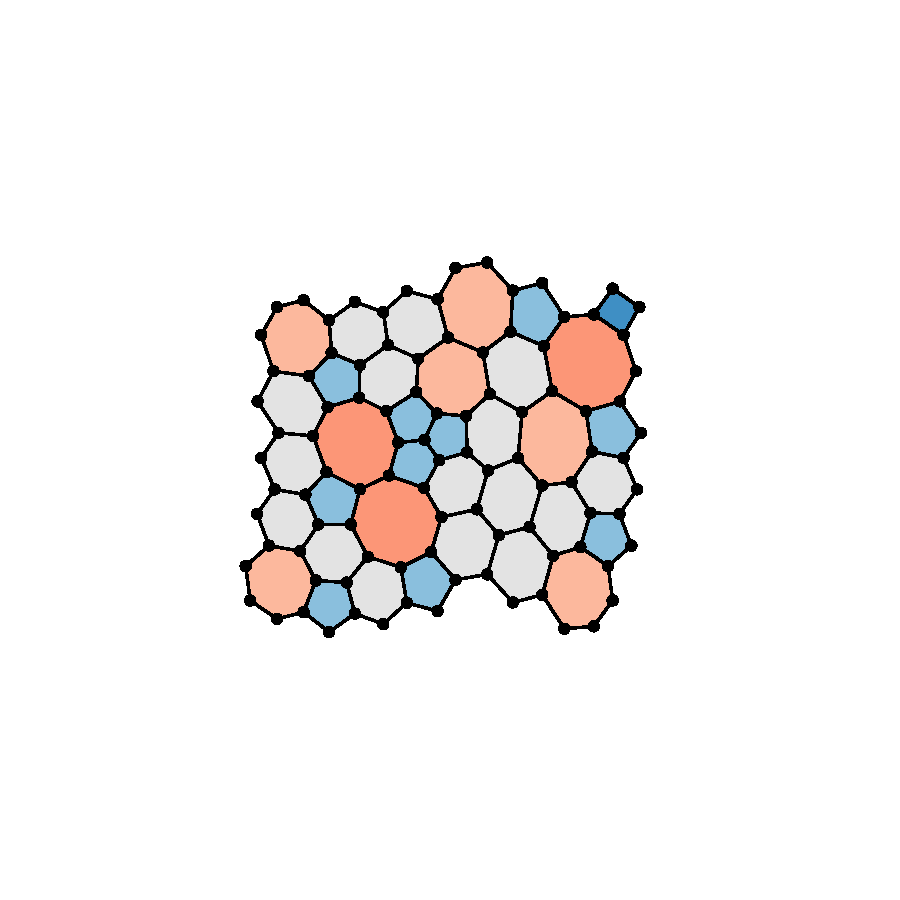
\includegraphics[width=\textwidth]{./figures/methods/graph.pdf}
         \caption{Atomic network}
         \label{fig:graphdualgraph}
     \end{subfigure}
     \hfill
	\begin{subfigure}[b]{0.3\textwidth}
         \centering
         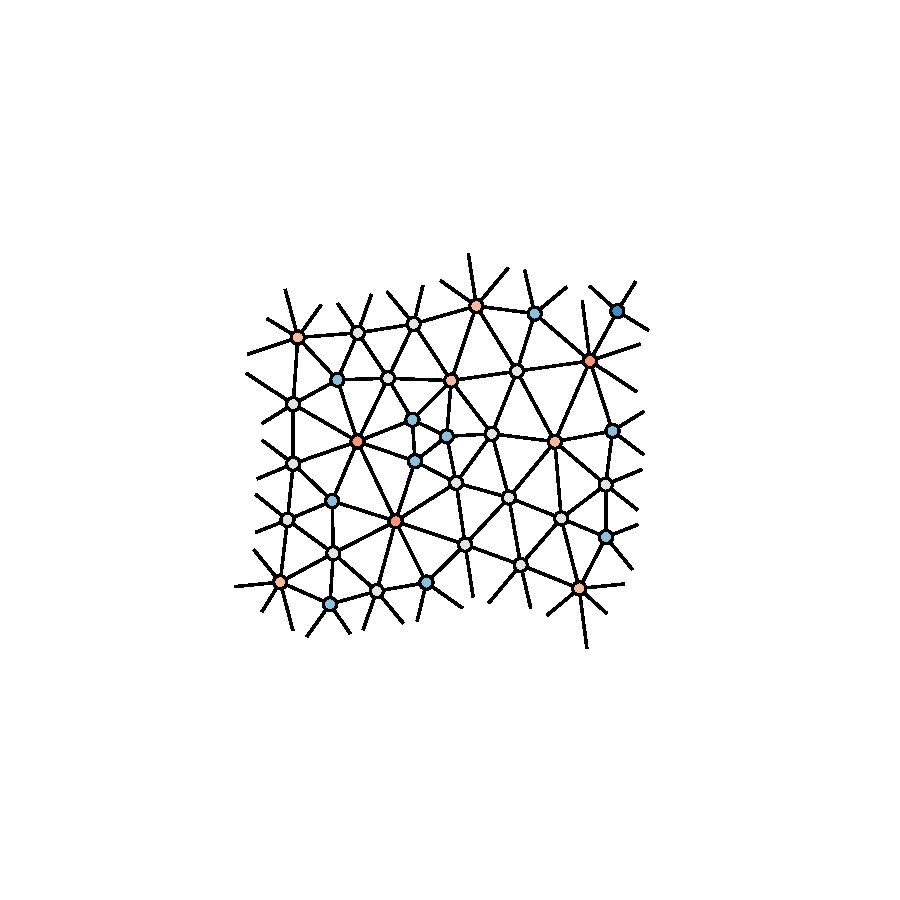
\includegraphics[width=\textwidth]{./figures/methods/dual.pdf}
         \caption{Ring network}
         \label{fig:graphdualdual}
     \end{subfigure}
     \hfill
     \begin{subfigure}[b]{0.3\textwidth}
         \centering
         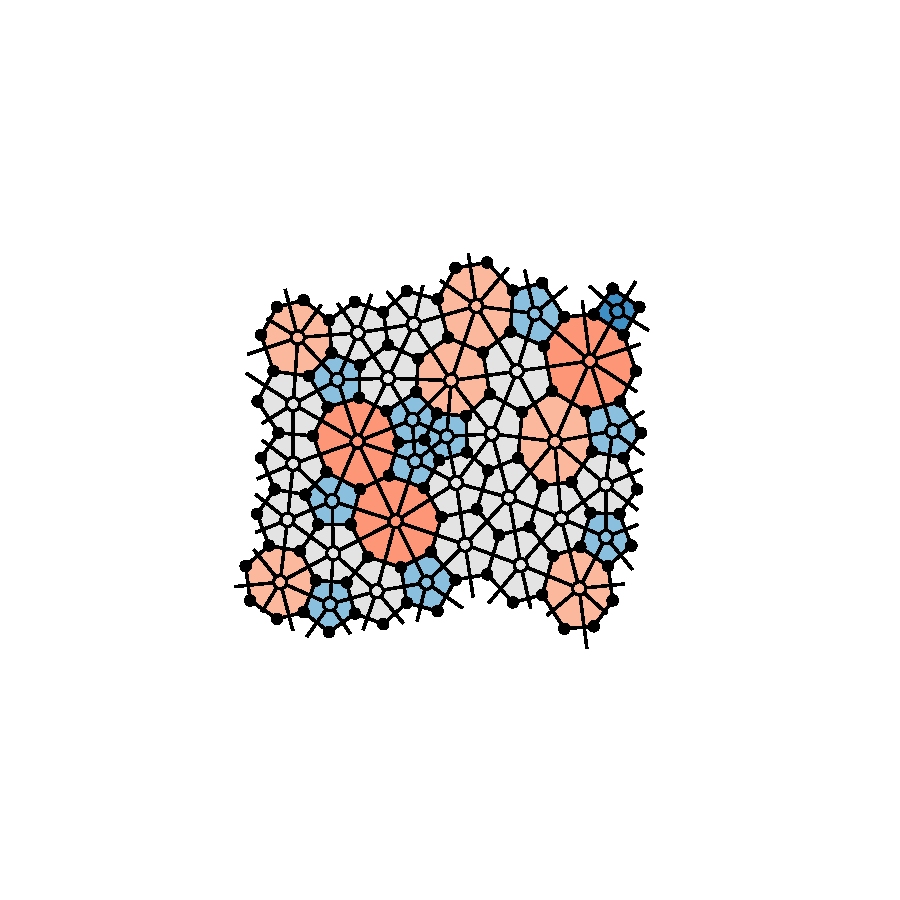
\includegraphics[width=\textwidth]{./figures/methods/graph_dual.pdf}
         \caption{Dual relationship}
         \label{}
     \end{subfigure}
     \hfill
     
     \caption{Panel (a) gives an example of a 3\-- coordinate periodic atomic network with disordered ring structure. Nodes and links represent atoms and bonds respectively where rings are coloured by size. Panel (b) gives the corresponding ring network where nodes and links represent rings and their adjacencies, where nodes are coloured by degree. Panel (c) shows the dual relationship between the atomic and ring networks, where the node degree in the ring network is equal to the ring size in the atomic network.}
     \label{fig:graphdual}
\end{figure}

Observing figure \ref{fig:graphdualgraph} one can see there is another level of structure in the network, namely that of the ring structure.
A ring is strictly any closed path of sequentially linked nodes in a network, but this thesis will use the term in reference only to the primitive rings \ie{} those which cannot be subdivided into two smaller rings \cite{Yuan2002}.
A ring of size $k$ (or $k$\--ring) is then defined as a ring with $k$ constituent nodes.
It is clear that finding and counting the number of rings of each size, often termed calculating the ring statistics, does then quantify the disorder in the system \cite{Kumar2014}.
The ring statistics can be summarised by the normalised probability distribution, $p_k$.

However, there is a more efficient way of representing and quantifying the ring structure in the system, and that is by constructing the dual network \cite{Aboav1984}.
The dual is generated by placing a node at the centre of each ring and linking the nodes of adjacent (\ie{} edge\--sharing) rings, as can be seen in figure \ref{fig:graphdualdual}.
This will be referred to as the ring network.
The ring network is a reciprocal lattice in which the node degree, $k$, is equivalent to the ring size in the atomic network.
Similarly, it consists solely of triangles, reflecting the 3\--coordinate nature of the underlying atomic network.
Hence, the disorder is captured directly in the node properties of the ring network.
These characteristics make the ring network preferable for manipulating and analysing the systems in this thesis.

\section{Topological Laws}
\label{s:topolaws}

There are a number of laws which govern the topological properties of \td{} network\--forming materials.
These laws constrain the ring structure, influencing the network properties in a manner that makes physical networks unique in the field of network science.
These laws act on a number of ``levels'': Euler's law controls the overall mean ring size, \lm's{} law the ring size distribution and the \aw{} law the ring\--ring correlations.

\subsection{Euler's Law}
\label{s:eulerslaw}

Euler's law constrains the mean ring size, $\ki$, in an atomic network or equivalently the mean node degree of the ring network.
The atomic networks studied in this work are all \td{}, connected (there is a path between any two nodes) and planar (they have no overlapping links) and so are subject to Euler's formula which states:
\begin{equation}
	\label{eq:eulerformula}
	N + V - E = \chi,
\end{equation}
where $N$, $V$, $E$ are the number of rings, vertices and edges in the network and $\chi$ in an integer termed the Euler characteristic, which is dependent on the global topology of the system.
Each vertex represents an atom and the number of edges emanating from each vertex is then the coordination number.

For generality consider an atomic network with atoms of assorted coordination numbers, $c$. 
If the proportion of each coordination type is $x_c$, then the mean coordination number is given by $\langle c \rangle = \sum\limits_c cx_c$.
This allows the number of edges to be written in terms of the number of vertices as $E=\frac{V}{2}\langle c \rangle$. 
In turn the mean ring size is simply the total number of vertices per ring, allowing for multiple counting, such that $\ki=\frac{V}{N}\langle c \rangle$.
Substituting these two expressions into equation \eqref{eq:eulerformula} leads to the expression:
\begin{equation}
	\label{eq:avdegree}
	\ki = \frac{2\langle c \rangle\left(1-\chi/N\right)}{\langle c \rangle - 2}.
\end{equation}
Hence the average node degree in the ring network (equivalent to the mean ring size of the physical network), is simply related to the average degree of the physical network (\ie{} local coordination environment), the topology of the system and the number of rings.

Although equation \eqref{eq:avdegree} may appear simple, it is a very powerful constraint. 
To demonstrate this consider a two\--dimensional lattice with two possible coordination environments $c=3,4$. 
The planar case with periodic boundary conditions (mimicking an infinite planar lattice) maps onto the torus with $\chi=0$, and so:
\begin{equation}
	\label{eq:2dplanarcases}
	\ki = \begin{cases}
		6, \quad x_3 = 1 \\
		4, \quad x_4 = 1 \\
		5, \quad x_3 = 2/3, x_4 =1/3
	\end{cases}\,.
\end{equation}
To reiterate in plain terms, this means that if there is a material consisting of atoms all forming exactly three bonds (as for amorphous carbon), the mean ring size \textit{must} be equal to six. 
Similarly if all atoms form four bonds the mean ring size is four, and if there is a two\--thirds to one\--third mixture of coordination environments the mean ring size is five.
The simplest illustrations of these are the hexagonal, square and cairo regular tilings, shown in figure \ref{fig:lattices}, but this law holds equally well for amorphous configurations.
For aperiodic systems strictly $\chi=1$, but as $N\rightarrow \infty$, the proportion of vertices with unsatisfied coordination on the sample perimeter become negligible overall as does the term in $\chi$.
Therefore in reality these relationships hold, and remain as applicable to amorphous graphene as the basalt columns in Fingal's Cave, and the Penrose tiling \cite{Goehring2014,Ressouche2009}.

This analysis also extends to spherical topology where $\chi=2$, and so:
 \begin{equation}
 	\label{eq:2dsphericalcases}
	\ki = \begin{cases}
		\frac{6N-12}{N}, \quad x_3 = 1 \\
		\frac{4N-8}{N}, \quad x_4 = 1.
	\end{cases}
\end{equation}
These relationships are the origin of the 12 pentagon rule for 3-coordinate fullerenes (the ``football problem''), or equivalently an ``8 triangle rule'' in the 4-coordinate case, as this is the only way to satisfy these equations if the allowed ring sizes are limited to $k=5,6$ and $k=3,4$ respectively (as in figures \ref{fig:latticesfull92}, \ref{fig:latticesfull98}) \cite{Fowler1996}.
Much of the richness in the behaviour of \td{} physical networks stems from this fundamental constraint on the network average degree.

\begin{figure}[bt]
     \centering
     
     \begin{subfigure}[b]{0.3\textwidth}
         \centering
         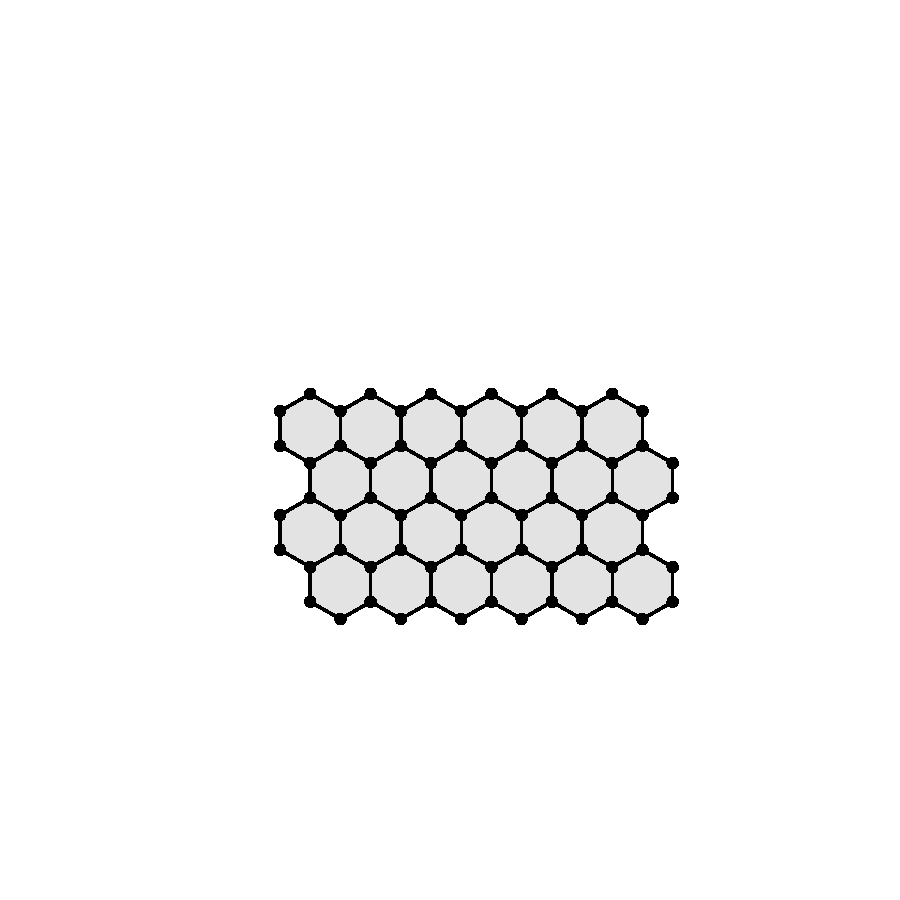
\includegraphics[height=2.4cm]{./figures/methods/hex.pdf}
         \caption{Hexagonal}
         \label{fig:latticeshex}
     \end{subfigure}
     \hfill
     \begin{subfigure}[b]{0.3\textwidth}
         \centering
         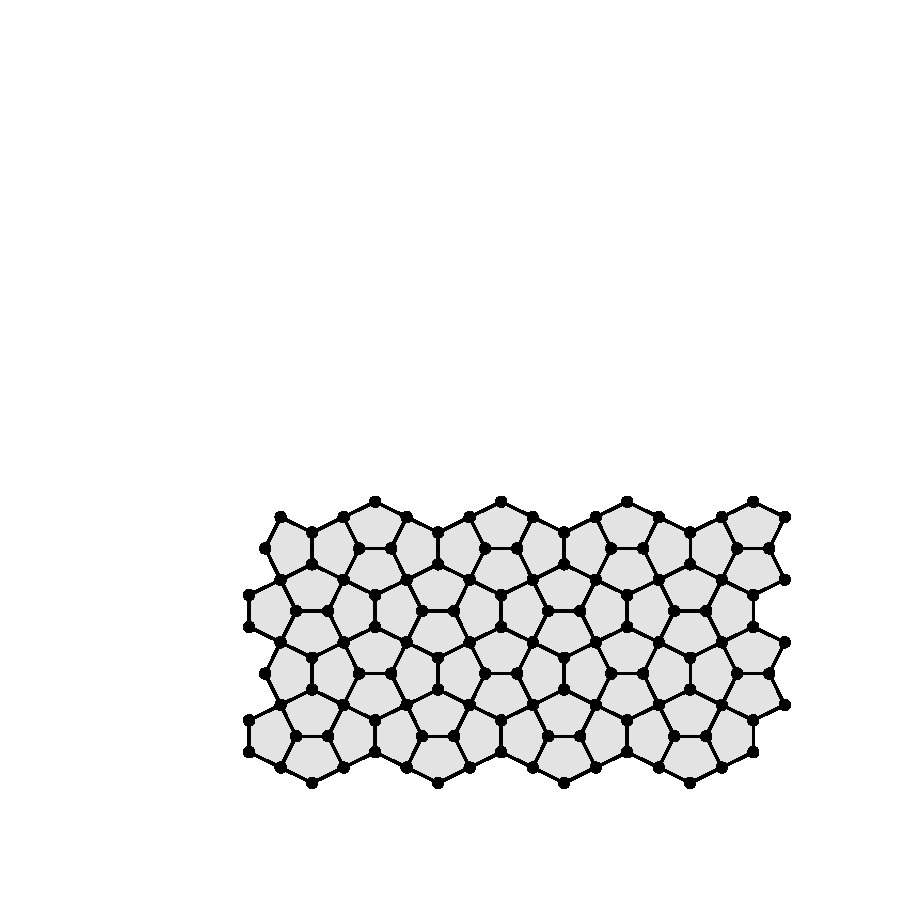
\includegraphics[height=2.4cm]{./figures/methods/cai.pdf}
         \caption{Cairo}
         \label{fig:latticescairo}
     \end{subfigure}
     \hfill
	\begin{subfigure}[b]{0.3\textwidth}
         \centering
         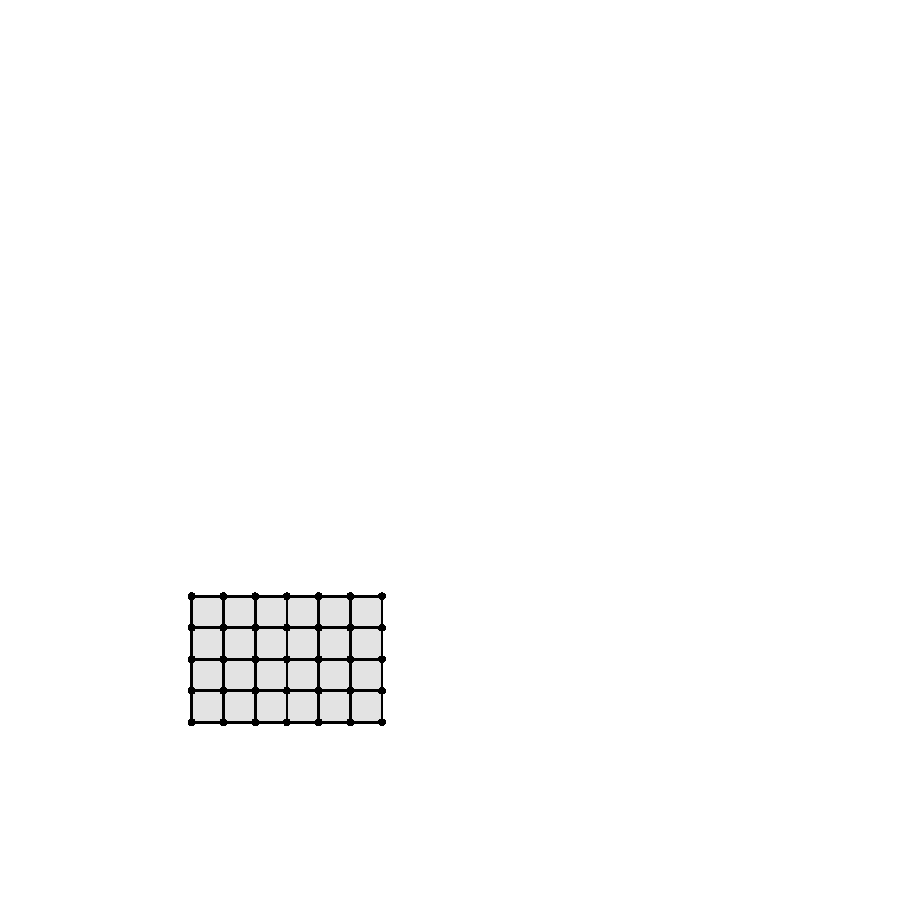
\includegraphics[height=2.4cm]{./figures/methods/sq.pdf}
         \caption{Square}
         \label{fig:latticessq}
     \end{subfigure}
     \hfill
     \vspace{0.5cm}
     
       \begin{subfigure}[b]{0.45\textwidth}
         \centering
         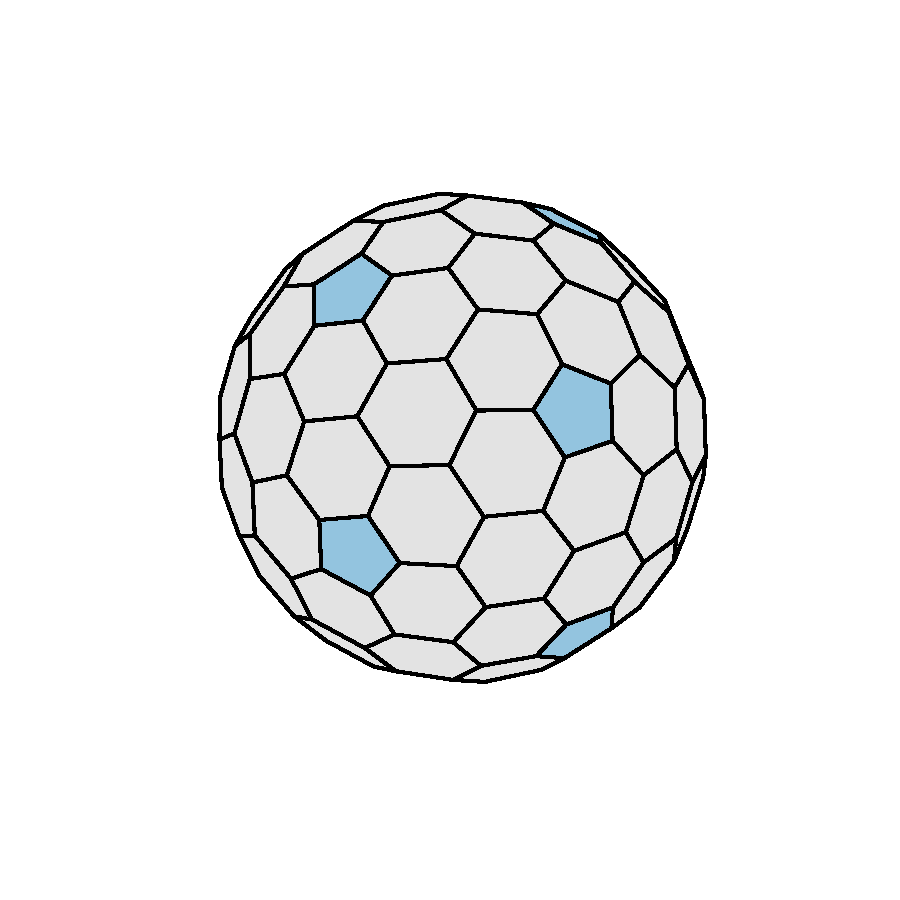
\includegraphics[height=2.4cm]{./figures/methods/full92.pdf}
         \caption{3\--coordinate fullerene}
         \label{fig:latticesfull92}
     \end{subfigure}
     \hspace{1cm}
     \begin{subfigure}[b]{0.45\textwidth}
         \centering
         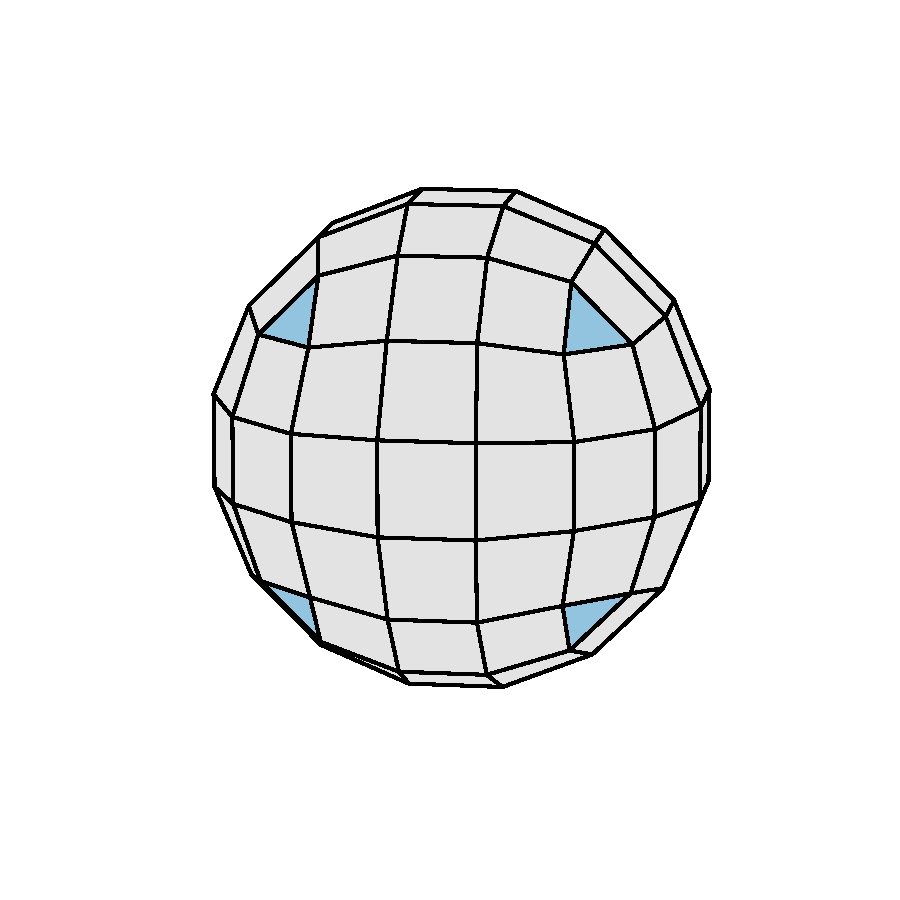
\includegraphics[height=2.4cm]{./figures/methods/full98.pdf}
         \caption{4\--coordinate fullerene}
         \label{fig:latticesfull98}
     \end{subfigure}
     
     \caption{Panels (a)\--(c) give regular planar tilings of 6\--, 5\-- and 4\-- rings, where the ring size is related to the underlying atomic coordination. Panels (d) and (e) show the 3\-- and 4\-- coordinate tilings in spherical topology, where the mean ring size is reduced due to the change in the Euler characteristic.}
     \label{fig:lattices}
\end{figure}

\subsection{\lm's Law}
\label{s:lemaitre}

Knowing that the mean node degree is fixed by Euler's law, the next level of available information is the form of the underlying degree distribution, $p_k$.
Interestingly, the degree distributions found in physical ring networks seem relatively well defined.
For instance, it has been noted in models and realisations of \td{} silica glass that the ring statistics looked to follow a lognormal distribution \cite{Shackelford1981,Buchner2017}.
\lm{} \etal{} demonstrated that the distribution in 3-coordinate networks systems can be well described by a maximum entropy distribution \cite{Gervois1992}.
\lm's{} maximum entropy method is summarised here, trivially extended to arbitrary coordination.

The entropy of a probability distribution is defined as 
\begin{equation}
	\mathcal{S}=-\sumk p_k\log p_k. 
\end{equation}
In addition, the degree distribution has the following constraints:
\begin{align}
		\sumk p_k &=1, \\
		\sumk kp_k&=\ki,  \label{con:lm2}\\
		\sumk \frac{p_k}{k}&=\text{constant} \label{con:lm3},
\end{align}
where the first two constraints correspond to the normalisation condition and the fixed mean ring size, and the final constraint will be discussed below.
The entropy can then be maximised using Lagrange's method of undetermined multipliers to yield the result:
\begin{equation}
	\label{eq:mepk}
	p_k = \frac{e^{-\lambda_1 k - \lambda_2 / k}}{\sumk e^{-\lambda_1 k - \lambda_2 / k}},
\end{equation}
which can be solved numerically by substitution into equations \eqref{con:lm2},\eqref{con:lm3}. 
By allowing the chosen constant to vary, a family of maximum entropy curves can be generated, as in figure \ref{fig:lm1}.
The resulting distributions can be summarised by relating the variance, $\mu_2=\kii-\ki^2$, to a single chosen node degree probability, leading to the plot known as \lm's law, given in figure \ref{fig:lm2}.
It is usually framed in the context of the proportion of hexagons in a system, $p_6$, for the precise reason that most networks have $\ki=6$ and $p_6$ as the largest contribution.
Many experimental and theoretical studies have shown good agreement to this law \cite{Caer1993,Cerisier1996,Miklius2012}.

Simple extensions of the classic law are however possible, by modifying the mean degree or the permitted degree range.
For instance, $k$ is usually taken in the interval $k\geq3$ (as the triangle, $k=3$, is the smallest polygon), but there can be manifestations of physical systems where only certain degrees are accessible \cite{Rivier1988}.
Additional examples of such systems will be procrystalline lattices explored in chapter \ref{ch:procrystals}. 
The resulting \lm{} curves for a selection of these modifications are given in figure \ref{fig:lm3}. 
A discussion of these will be recur throughout this thesis, but one can see that the application of the allowable ring size constraints leads to marked differences in the maximum entropy solutions.
The maximum value of these curves can be simply determined by removing constraint \eqref{con:lm3}, equivalent to setting $\lambda_2=0$ in equation \eqref{eq:mepk}.
%Exploring these cases helps to understand the behaviour of \lm's law itself.
%By restricting the ring size to just $5\leq k \leq 7$ results in a straight line, which to satisfy Euler's law must have equation $\mu_2 = 1-p_6$.
%This line closely follows the high $p_6$ behaviour demonstrating that the initial deviation from the hexagonal lattice ($p_6=1$) is marked by the introduction of 5\-- and 7\-- ring defects.


\begin{figure}[bt]
     \centering
     
     \begin{subfigure}[b]{0.45\textwidth}
         \centering
         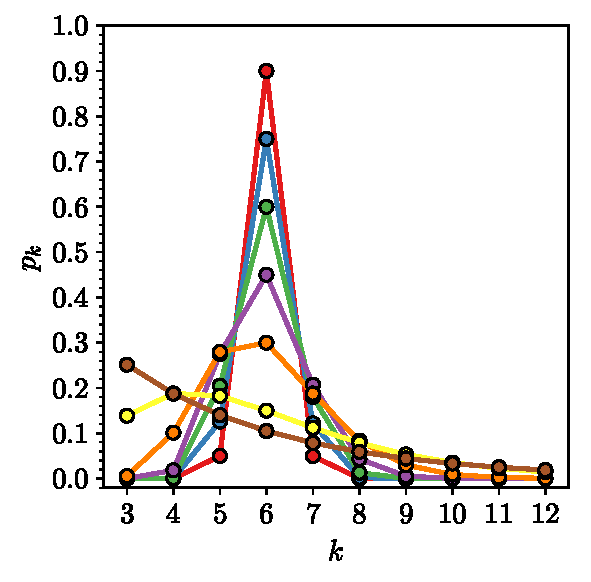
\includegraphics[width=\textwidth]{./figures/methods/lm_1.pdf}
         \caption{Maximum entropy distributions}
         \label{fig:lm1}
     \end{subfigure}
     \hfill
      \begin{subfigure}[b]{0.45\textwidth}
         \centering
         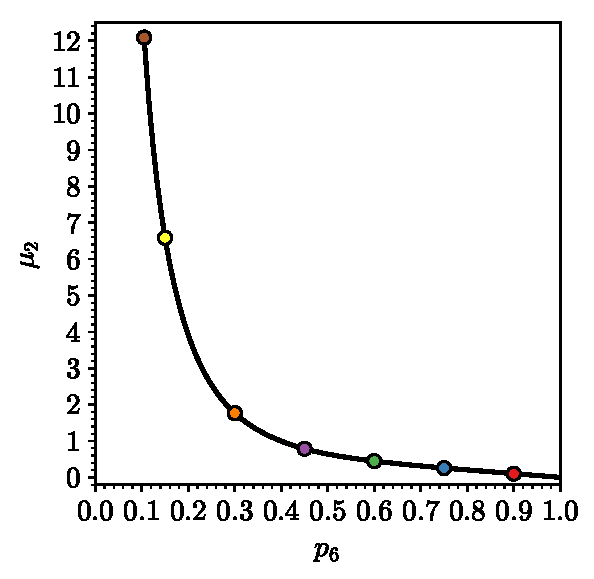
\includegraphics[width=\textwidth]{./figures/methods/lm_2.pdf}
         \caption{\lm's law}
         \label{fig:lm2}
     \end{subfigure}
     \hfill
     
      \begin{subfigure}[b]{0.45\textwidth}
         \centering
         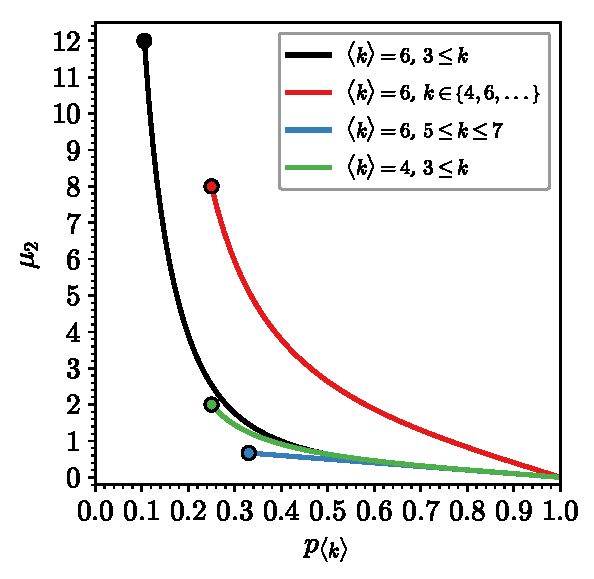
\includegraphics[width=\textwidth]{./figures/methods/lm_3.pdf}
         \caption{Extensions to \lm's law}
         \label{fig:lm3}
     \end{subfigure}
     \hfill

    
     \caption{Illustration of \lm's maximum entropy method. Panel (a) gives examples of explicit maximum entropy distributions with different values of $p_6$. Panel (b) shows how these distributions can be summarised in a plot of $p_6$ \vs{} $\mu_2$ (\lm's law). Panel (c) provides extensions to the law by modifying the underlying constraints of the mean ring size and allowable $k$\--range.}
     \label{fig:lm}
\end{figure}

The only somewhat puzzling aspect of this successful theory is the choice of constraint \eqref{con:lm3}.
It was originally rationalised on the basis that the areas of rings of a given size, $A_k$, can be well fit by an expression $A_k = ak+b+c/k$, where $a$, $b$ and $c$ are constants.
As noted at the time, this is by no means true for all systems and in fact is contrary to the widely known Lewis law, which states that $A_k$ is linear in $k$ for many observable networks \cite{Lewis1928,Fortes1995,Kim2014}.
Despite this, the universality of the \lm{} law suggests that there must be a physical basis to \eqref{con:lm3}, and in the section \ref{s:assortativity} it will be demonstrated that it can be regenerated by considering ring adjacencies.

\subsection{\aw{} Law}
\label{s:awlaw}

The ring statistics given by \lm's law are an important measure for physical networks, but they do not provide a complete characterisation of the ring structure, as they say nothing about the ring adjacencies. 
This is important because whilst with the same ring statistics it is theoretically possible to organise the rings in many different arrangements, it is well known experimentally that only a subsection of these are observed.
The vast majority of physical systems have a preference for small rings ($k<\ki$) be adjacent to large rings ($k>\ki$).
This effect was first noted in the grains of polycrystals by Aboav \cite{Aboav1970}.
Aboav quantified these ring correlations by measuring the mean ring size about a $k$\--ring, denoted $m_k$, and found empirically that $m_k \approx 5 + 8/k$.

In an attempt to explain this observation, Weaire came across the following relation
\begin{equation}
	\label{eq:weairesumrule}
	\sumk km_kp_k = \sumk k^2p_k = \mu_2 + \ki^2 \,,
\end{equation}
known as Weaire's sum rule \cite{Weaire1974}.
From this he suggested the modification of $m_k=5+\left(6+\mu_2\right)/k$ which satisfied this rule.
Aboav's original equation then became a special case when $\mu_2=2$, which is close to the expected value for a random collection of Voronoi polygons (see section \ref{s:voronoiintro}).
Aboav then proposed that if a generic form of $m_k = A + B/k$ was used in conjunction with Weaire's sum rule then
\begin{equation}
	m_k = A+\frac{\mu_2+\ki^2-A\ki}{k}\,.
\end{equation}
This is now more commonly expressed in the linear form \cite{Chiu1995}:
\begin{equation}
	\label{eq:aboavweaire}
	km_k = \mu_2+\ki^2+\ki\left(1-\alpha\right)\left(k-\ki\right).
\end{equation}
Equation \ref{eq:aboavweaire} is known as the \aw{} law and relates the mean ring size about a given central ring to a single fitting parameter, $\alpha$.
The value of $\alpha$ describes the strength of the ring correlations, with a larger positive value indicating a greater tendency for small\--large ring adjacencies.
More specifically, the random limit can be deduced by evaluating $\frac{\partial{m_k}}{\partial{x}}=0$ as \cite{Delannay1994}:
\begin{equation}
	\label{eq:awrandlim}
	\alpha=-\frac{\mu_2}{\ki^2} \,.
\end{equation}
Hence all systems with $\alpha>-\mu_2/\ki^2$ have more small\--large ring  adjacencies than would be expected from chance whilst conversely those with $\alpha<-\mu_2/\ki^2$ have more small\--small and large\--large pairings.

\begin{figure}[tb]
     \centering
      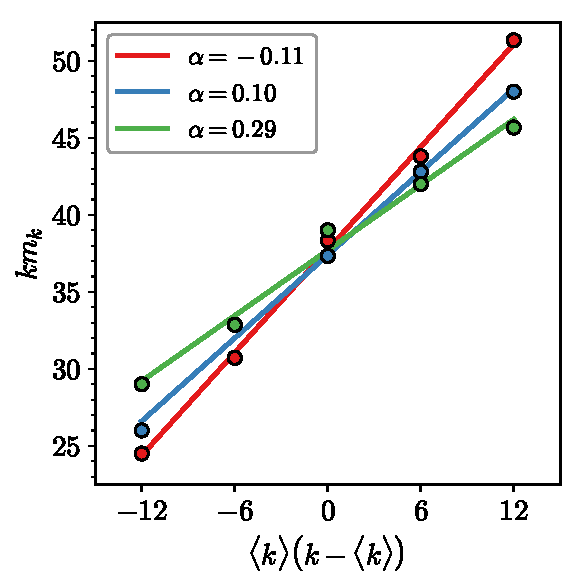
\includegraphics[width=8cm]{./figures/methods/aw_demo.pdf}
     \caption{Calculation of an \aw{} fit for three configurations (shown in figure \ref{fig:zach}(b)\--(d)). The value of the $\alpha$ parameter quantifies the tendency of small rings to be adjacent to large rings, with a larger value indicating stronger small\--large ring correlations.}
     \label{fig:awdemo}
\end{figure}

Despite the \aw{} law being purely empirical and there being no topological requirement for $m_k$ to vary systematically $k$, the law does seem to hold well for a diverse set of physical systems.
The law is well used for example in studies of materials, emulsions, biological tissues as well as in planetary science \cite{LeRoux2013,Roy2018,Noever1992,Mombach1993,Pedro2008}.
As an example of the calculation of the \aw{} parameter, the plots of the fits for the systems in figure \ref{fig:zach} are presented in figure \ref{fig:awdemo}, along with the corresponding $\alpha$ parameters.
This demonstrates two contrasting aspects of the \aw{} law. 
Firstly the law holds very well, especially given the fact that these samples consist of just twenty rings each.
However, it also demonstrates that the law is by no means exact and that some greyness is inevitably introduced during the linear regression.

